\chapter{Diffusion Map} 
\label{appendix-diffmap} 

Besides tensor CP decomposition, we also explore the non-linear dimensionality reduction method of diffusion map. (Note that most of the results presented in this report can be obtained from tensor CP decomposition. However, when the former failed to provide meaningful results, we turn to the diffusion map.) The main references for this section are \cite{coifman_geometric_2005},   \cite{coifman_diffusion_2006} and \cite{stanley_geometric_2020}. We will now outline the steps in the diffusion map algorithm.
\begin{enumerate}
\item Discretize the underlying manifold as a weighted graph.
\begin{defn}[Discretization of a manifold]

Given $X = \{x_1, x_2,\dots, x_n\}$, a set of data sampled from a Riemannian manifold $\mathcal{M}$, we can construct the discretization of $\mathcal{M}$ as as a weighted, undirected graph, $\mathcal{G}_X = (X, g_\epsilon)$ where $X$ is the set of vertices given by the data and $g_\epsilon$ is a Gaussian kernel function $g_\epsilon: (x_i, x_j) \to [0,\infty]$ defined by the following rule
\begin{align}
    g_\epsilon(x_i,x_j) = \frac{1}{2}\left(\exp{\frac{-\|x_i - x_j\|_2^2}{2\epsilon(x_i)}} + \exp{\frac{-\|x_i - x_j\|_2^2}{2\epsilon(x_j)}}\right), \quad \forall x_i,x_j \in X, 
\end{align}

 where $\epsilon: X \to \RR$ is the the bandwidth function by which the Gaussian kernel is parameterized. 
\end{defn}

Gaussian kernel is only one of the possible kernel functions, but it gives a physically intuitive construction for learning the manifold underlying the data sample because it effectively considers a ball of radius $\epsilon$ around each data point.

The choice of $\epsilon$ determines the radius of neighborhood of $x_i \in X$. $\epsilon$ is application-specific and is usually a global bandwidth, that is, $\epsilon(x_i) = \epsilon(x_j)$ for all $x_i, x_j \in X.$ 

\item Compute the similarity matrix associated with the weighted graph.

Given the weighted graph $\mathcal{G}_X$, we can compute the corresponding similarity matrix. Each entry in the similarity matrix, $W_{i j}$, is the pairwise similarity value between data/vertices $x_i$ and $x_j$ and is taken as the weight of the edge between nodes $x_i$ and $x_i$. 
    \begin{align}
        W_{i j } = \exp\{-\frac{\|x_i - x_j\|^2}{2\sigma^2}\}.
    \end{align}
    
\item Construct a lazy random walk on $\mathcal{G}_X$. 

First, we define random walk on the weighted, undirected graph $\mathcal{G}_X$: 

\begin{defn}[Random walk on graphs]
A \underline{random walk} on $\mathcal{G}_X = (X,g_\epsilon)$ is a process that begins at some vertex $x_i$, and at each time step moves to another vertex $x_j$. Since the graph is weighted, it moves to a neighbor $x_j$ with probability $p(j \mid i)$, proportional to the weight of the corresponding edge, and is defined as follows:
\begin{align}
        p(j\mid i) = \frac{W_{i j}}{\sum_{k} W_{i k}}.
\end{align}
The random walk is \underline{lazy} if we allow $p(i\mid i) > 0$, i.e., the probability of staying at some point $i$ as the time step moves forward is non-zero.
\end{defn}
    
    The probabilities $p(j \mid i)$ can be represented by a Markov matrix $M$, which is essentially the similarity matrix normalized to have row sums equal to $1$:
     \begin{align}
        M = D^{-1} W, \text{where } D_{i i} =\sum_{k}W_{i k}.
    \end{align}
    The probability of reaching node $x_j$ from $x_i$ after $t$ steps is then
    \begin{align}
        p(t,j\mid i) = e_i^T M^t e_j.
    \end{align}

    \item Eigendecomposition of the Markov matrix:
    
    The eigendecomposition of $M$ is derived from the eigendecomposition of $M_s = D^{1/2} M D^{-1/2} = \Omega \Lambda \Omega^T$:
    \begin{align}
        M = D^{-1/2}  \Omega \Lambda \Omega^T D^{-1/2} \coloneqq \Psi \Lambda \Phi^T.
    \end{align}
    
    Note that since $\Psi$ and $\Phi$ are mutually orthogonal, $\Psi$ contains the right eigenvectors, as shown below:
     \begin{align}
        M \Psi =  \Psi \Lambda \Phi^T \Psi = \Psi \Lambda =  \Lambda \Psi.
    \end{align}
    
    The eigendecomposition of $M$ after $t$ steps is then
    \begin{align}
        M = \Psi \Lambda^t \Phi^T.
    \end{align}
    \begin{itemize}
        \item Diffusion coordinate functions are the right eigenvectors of Markov matrix scaled by their corresponding eigenvalues: 
        \begin{align}
            \Upsilon \coloneqq \Psi \Lambda.
        \end{align}
        \item Diffusion distance after $t$ steps is the following:
       \begin{align}
            \| e_i^T  \Upsilon - e_j^T \Upsilon  \|^2 = \sum_{k} (p(t,k\mid i) - p(t,k\mid j))^2 (D_{k k}^{-1}).
       \end{align}
       
       \item Infer geometric properties from the growth of eigenvalues of $M$.
       
       For intuition behind the relation between the growth of eigenvalues and the geometric properties of the underlying manifold that we begin with, we consider the following two extreme situations:
       \begin{enumerate}
           \item If the discretization of the underlying manifold is a disconnected graph (none of the nodes are connected), then:
           \[P = I, \lambda_i = \lambda_j \quad \forall i, j, \]
           which implies a flat spectrum with zero decay rate.
           \item If the discretization of the underlying manifold is a fully connected graph (each of the node is connected to all the rest of the nodes), assuming weights of all edges are $1$, then:
            \[\lambda_1 = 1, \lambda_i = 0 \quad \forall i \neq 1.\]
       \end{enumerate}
    \end{itemize}
\end{enumerate}

\par \textbf{Key ideas of diffusion maps: }
\begin{itemize}
    \item The similarity kernel gives us the \textit{local} geometry. As the time steps move forward, we integrate the local geometry and thus reveal the geometric structures at different scales. 
    \item A cluster from a random walk is a region where the probability of escaping this region is low.
\end{itemize}

\section{Demonstration of the method}
As a demonstration of the diffusion maps method, we apply it on synthetic spiral data and MNIST handwritten digits images data:

\begin{figure}[H]
        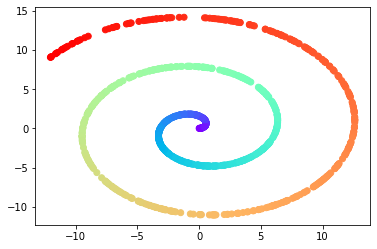
\includegraphics[width=0.6\textwidth]{presentation/spiral.png}
        \caption{Visualising the original spiral data.}
    \end{figure} 
  \begin{figure}[H]         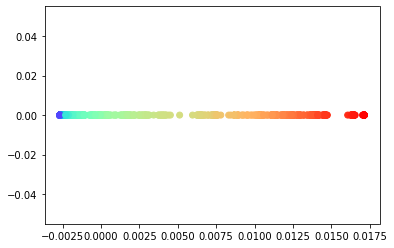
\includegraphics[width=0.6\textwidth]{presentation/spiral-unroll.png}
        \caption{First non-trivial coordinate function.}
        \end{figure} 
\begin{figure}[H]
        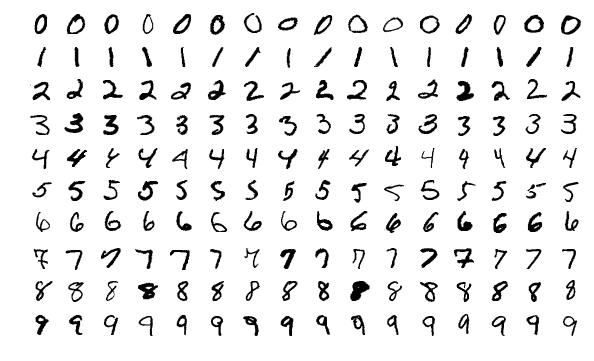
\includegraphics[width=0.4\textwidth]{presentation/mnist-vis.png}
        \caption{Sample data from the MNIST.}
    \end{figure} 
  \begin{figure}[H]
            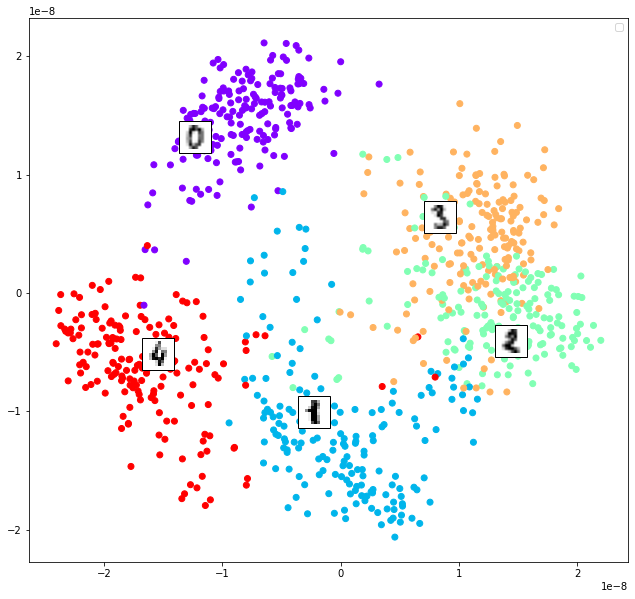
\includegraphics[width=0.6\textwidth]{presentation/mnist.png}
        \caption{First two non-trivial coordinate functions (plotting only five of the digits classes).}    
        \end{figure} 
        
\section{Remarks on non-linear dimensionality reduction}
Setting the right parameters for non-linear dimensionality reduction is very challenging, especially for lab data where sampling errors are prevalent. For this reason, we will be investigating this method in greater details in the second half of the project instead.  

% [to-do: axis set to equal for the plot; and mention only plotting 5 classes]